\documentclass[paper=a4, fontsize=12pt]{article}
\usepackage[margin=1.2in]{geometry}
\usepackage[T1]{fontenc}
\usepackage{fourier}
\usepackage{hyperref}
\usepackage[english]{babel}
\usepackage[protrusion=true,expansion=true]{microtype}				
\usepackage{amsmath,amsfonts,amsthm}									
\usepackage{graphicx}
\usepackage{natbib}											
\usepackage{sectsty}												
\allsectionsfont{\centering \normalfont\scshape}
\usepackage{fancyhdr}
\pagestyle{fancyplain}
\fancyfoot[C]{Prof. Dr. Adalbert F.X. Wilhelm\\JTBU-020003 $:$ Big Data: Big Boon and Big Brother}

\newcommand{\horrule}[1]{\rule{\linewidth}{#1}} 	
\title{
		\vspace{-1in} 	
		\usefont{OT1}{bch}{b}{n}
		\normalfont \normalsize \textsc{School of Humanities and Social Sciences\\Jacobs University Bremen} \\ [25pt]
		\horrule{0.5pt} \\[0.4cm]
		\huge Debating the ethical and technological challenges surrounding open access to clinical trial data\\
		\horrule{2pt} \\[0.5cm]
}
\author{Nick Lee\\Rashed Popalzai\\Siddharth Shukla\\Trang Le\\\\\today}
\date{}
\begin{document}
\maketitle
\newpage
\fancyhead[C]{Nick Lee $\cdot$ Rashed Popalzai $\cdot$ Siddharth Shukla $\cdot$ Trang Le $\cdot$ Jacobs University Bremen}


\section*{Background}
Clinical trials are a set of experiments in research studies that investigate whether specific pharmaceuticals, medical treatment strategies, medical devices are safe and effective for human use. In clinical studies, human volunteers are given certain interventions according to protocols and plans set up by the investigators. These interventions might be a new drug, device, procedure, or change in diet. \\\\
In the past few decades, clinical trial study results as well as their associated databases have been growing not only in volume but also in diversity and in incongruity. This is especially aided by the evolution of ?omics? data at individual patient level: genomics, proteomics, transcriptomics and metabolomics to name a few, not to mention the information about background history of patient populations like demographics, epidemiology, family history, lifestyle.\\\\
Sharing of such valuable data can enhance the understanding of the complex medical problem by combining multiple study results and perform meta-analysis to extend scientific findings beyond the original theory. Even incomplete or failed clinical trial can be extremely useful in avoiding similar mistakes. In the USA, the efficiency, accuracy and timely data is a concern. In this project we will focus on how the clinical trial data is shared in the US and how is it contributing in improving the quality of the health care system.


\section*{Big Data Initiative}
Clinical trials require tremendous amount of time and funding, and produce as a result huge amount of relevant and irrelevant data. In order for the clinical trial data to be publicly available for the investigators, Networks need to be established and databases administered. \\\\
The Clinical Research Network (CRN) is, for example, designed to facilitate data sharing between the interested stakeholders. In the US, clinicaltrials.gov was developed by the  National Institute of Health (NIH) as a platform for the investigators to post their trial findings and for the public and other interested stakeholders to look into the data.\\\\
As shown in figure 1.1, the clinical trials registered in the database saw a dramatic increase from less than 2000 trials in 2004 and more than 13000 trials in 2005.\\
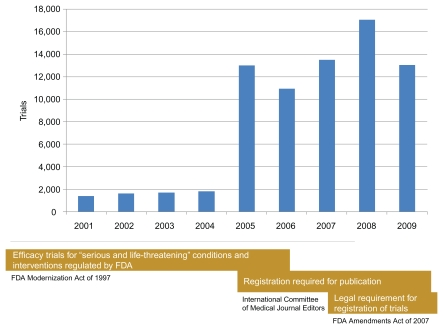
\includegraphics[width=\textwidth]{trialdata}\\
According to Krall there were 10,974 ongoing trials with at least one US center, totalling 2.8 million study subjects. (Transforming Clinical Research in the United States: Challenges and Opportunities: Workshop Summary, 2010).\\\\
Although \href{clinicaltrials.gov}{clinicaltrials.gov} is a good example of how to collect clinical trial data from different sources, it does not gaurantee the validity of the findings which makes it problematic for those looking for high quality data. The goal of the database is not effectiveness, that is how well they answer the research question but rather how efficiently they are conducted. 
Timeliness and variability of the data are other concerns regarding the \href{clinicaltrials.gov}{clinicaltrials.gov}.


\section*{Research question}
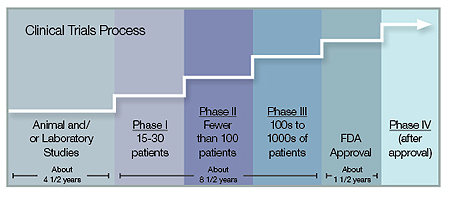
\includegraphics[width=\textwidth]{trialprocess}
Clinical trials are risky, complex and costly. For example, in drug development process, after several screenings for bioactive compounds, lead drug candidates are determined and run through more experiments in laboratory and animal studies. From those leads, new drugs are entered into clinical trial studies that can last for as long as 10 years while involving thousands of patients. If clinical trials prove successful, the drug may be certified for sale. Moreover, the failure rate is extremely high. This process takes around 15 years of work and hundreds of millions to billions of dollars to complete.\\\\
Besides the obvious potential knowledge can be withdrawn from such valuable information, the problems associated with data sharing and the complexity of data management are not to be underestimated.On this project we will try to look at the state of the clinical trials and try to answer some ethical questions regarding the morality of sharing the findings of the trials and how can it affect the individuals and groups participating in the studies. We will also talk about the clinical trials in the US and will try to answer how costly and effective it is to share clinical trial data and make it available to the public.\\\\


\section*{Project plan}
The project plan for this research project can be itemised in 7 week from now.\\
\begin{itemize}
\item{\emph{Week 1}} : Research multiple datasets and figure out what datasets are most optimal for the problem we?re looking to solve
\item{\emph{Week 2}} : Organise dataset such that insight into the data is possible, potentially transforming or simplifying it
\item{\emph{Week 3}} : Analyze the dataset to find pattern within the dataset
\item{\emph{Week 4}} : Make inferences from patterns within the dataset and draw preliminary conclusions and counterarguments
\item{\emph{Week 5}} : Verify the conclusions and start working on the deliverable
\item{\emph{Week 6}} : Visualize the data and conclusion (draft)
\item{\emph{Week 7}} : Visualize the data and conclusion (final), and present the research
\end{itemize}


\section*{References}
\begin{itemize}
\item Institute of Medicine (US) Forum on Drug Discovery, Development, and Translation. Transforming Clinical Research in the United States: Challenges and Opportunities: Workshop Summary. Washington (DC): National Academies Press (US); 2010. 2, The State of Clinical Research in the United States: An Overview.Available from: \href{http://www.ncbi.nlm.nih.gov/books/NBK50886}{http://www.ncbi.nlm.nih.gov/books/NBK50886}
\item The University of Texas MD Anderson Cancer Center, State of Texas. `Clinical Trial Phases : Cancer Research | MD Anderson Cancer Center'. \href{Mdanderson.org}{Mdanderson.org}. N.p., 2015. Web. 5 Oct. 2015.
\end{itemize}
\end{document}